\chapter{Metodologie di sviluppo}

\section{Ingegneria del Machine Learning}
Approcciarsi allo sviluppo di un progetto senza preoccuparsi della sua ingegnerizzazione è uno degli errori più comuni e pericolosi dello sviluppo del Software. Senza una precisa metodologia, infatti, risulta quasi impossibile realizzare un sistema software affidabile o che riesca a fornire le corrette funzionalità agli utenti. È quindi di fondamentale importanza scegliere e seguire un modello di sviluppo del software per evitare (o mitigare) questo tipo di problematiche.

\subsection{Il CRISP-DM}
Quanto detto vale per lo sviluppo di qualunque tipo di software. Tuttavia la realizzazione di un modello di Machine Learning introduce nuove problematiche di cui tenere conto. In particolare, a differenza dei sistemi software tradizionali, nel Machine Learning si fa uso di grandi quantità di dati ed è quindi cruciale preoccuparsi della loro qualità e gestione.

Di conseguenza sono due le cose principali a cui pensare quando si progetta una soluzione basata su Machine Learning: Ingegneria del Software e Ingegneria dei Dati.

Per questi motivi, il modello scelto per progettare AutoMate è il \mbox{CRISP-DM} (Cross-Industry Standard Process for Data Mining), un modello non sequenziale in cui le diverse fasi possono essere eseguite un numero illimitato di volte e che prevede sia i tradizionali processi di Software Engineering che quelli di Data Engineering.

\medskip
\pagebreak
\section{Risoluzione del problema}
Come precedentemente specificato, lo sviluppo del progetto seguirà il modello CRISP-DM. Di seguito sono riportate le fasi del modello, e per ciascuna di esse sono state dettagliatamente descritte le scelte e le operazioni effettuate per raggiungere con successo gli obiettivi prefissati.

\subsection{Business Understanding}
La fase di \textbf{Business Understanding} prevede, come tutte le fasi iniziali di un progetto software, attività di raccolta dei requisiti e definizione degli obiettivi di business che si intende raggiungere. Inoltre è necessario determinare la disponibilità delle risorse, stimare i rischi e selezionare le tecnologie e i tool necessari al raggiungimento degli obiettivi.

\paragraph{Obiettivi di business.}
AutoMate ha come obiettivo principe quello di conferire ai suoi utilizzatori uno strumento che sia in grado di stimare il valore di un'auto tenendo conto sia di caratteristiche più generali come marca e modello, sia di informazioni più specifiche come tipo di trasmissione, potenza e presenza di danni e/o difetti.

\paragraph{Disponibilità delle risorse.}
Come già discusso nella \hyperref[sec:problematicheDataset]{\textbf{Sezione 2.4}}
la bassa disponibilità di Dataset ha portato alla selezione di un insieme di dati non molto recente (i dati sono stati estratti nel 2016). Ciò non rappresenta un grosso problema dal punto di vista della realizzazione del modello poiché la struttura di un ideale Dataset più recente sarebbe abbastanza simile. Tuttavia ciò comporta un certo grado di inattualità che compromette l'utilizzo efficace di AutoMate in tempi odierni.

\paragraph{Stima dei rischi.}
Tra i possibili rischi che si potrebbero presentare è opportuno prestare particolare attenzione alle caratteristiche su cui la predizione sarà effettuata. Se non accuratamente selezionate, le features utilizzate per stimare il valore dell'auto potrebbero portare a risultati non corretti o comunque molto distanti dalla realtà.

\paragraph{Tecnologie e tool utilizzati.}
Per lo sviluppo del modello e le operazioni di acquisizione, analisi e modellazione dei dati verrà utilizzato il linguaggio \textbf{Python} e nello specifico le librerie \textbf{pandas}, \textbf{seaborn} e \textbf{Scikit-learn}.
\pagebreak

\subsection{Data Understanding}
La fase di \textbf{Data Understanding} si compone delle operazioni di identificazione, collezione e analisi dei Dataset che possono portare al raggiungimento degli obiettivi. Vengono infine identificati e discussi possibili problemi di qualità dei dati.

\paragraph{Identificazione e Collezione dei Dataset.}
Il Dataset selezionato per la risoluzione del problema è stato recuperato da \textbf{Kaggle}, una delle piattaforme più utilizzate nei campi della Data Science e del Machine Learning. Il Dataset è reperibile a questo link:
\textit{\url{https://www.kaggle.com/datasets/shaunoilund/auto-sales-ebay-germany-random-50k-cleaned}} %Rendere il link blu

\paragraph{Analisi dei Dataset.}
Il Dataset utilizzato contiene oltre 37.000 inserzioni di auto caricate su eBay Kleinanzeigan da utenti privati ed è rappresentato da un file in formato .csv (Comma-Separeted Values) all'interno del quale ogni record è descritto da valori separati da virgola.

Il Dataset presenta 18 campi, i quali vengono riportati di seguito con una breve descrizione:

\begin{itemize}
    \item \textbf{id}: identificativo dell'inserzione;
    \item \textbf{data\textunderscore crawled}: data di estrazione dell'inserzione.
    \item \textbf{car\textunderscore name}: testo dell'inserzione.
    \item \textbf{price\textunderscore EUR}: prezzo dell'auto in euro.
    \item \textbf{ab \textunderscore test}: se l'inserzione è inclusa in un test A/B.
    \item \textbf{vehicle\textunderscore type}: tipo di veicolo.
    \item \textbf{registration\textunderscore year}: anno di immatricolazione del veicolo.
    \item \textbf{transmission}: tipo di trasmissione dell'auto.
    \item \textbf{power\textunderscore ps}: potenza dell'auto in cavalli (CV).
    \item \textbf{model}: modello dell'auto. 
    \item \textbf{odometer\textunderscore km}: chilometraggio dell'auto.
    \item\textbf{registration\textunderscore month}: mese di immatricolazione del veicolo.
    \item \textbf{fuel\textunderscore type}: tipo di carburante dell'auto.
    \item \textbf{brand}: marca dell'auto.
    \item \textbf{unrepaired\textunderscore damage}: presenza di danni non riparati all'auto.
    \item \textbf{date\textunderscore created}: data di creazione dell'inserzione.
    \item \textbf{postal\textunderscore code}: codice postale della locazione dell'auto.
    \item \textbf{last\textunderscore seen\textunderscore online}: data dell'ultima visita da parte del crawler.
\end{itemize}
Come si può notare, alcuni dei campi sopraelencati forniscono informazioni soltanto sull'annuncio dell'auto e non sull'auto stessa: non saranno pertanto presi in considerazione.

Per quanto riguarda i restanti attributi, grazie all'uso delle librerie \mbox{Python} \textbf{pandas} e \textbf{seaborn}, sono state effettuate operazioni di esplorazione dei dati al fine di visualizzarli e rilevare eventuali relazioni.

I risultati più interessanti dell'esplorazione sono di seguito riportati e discussi.
\bigskip

\lstset{language=Python}
\lstset{frame=lines}
\lstset{caption={\textbf{Codice utilizzato per l'esplorazione dei dati.}}}
\lstset{label={lst:codice}}
\lstset{basicstyle=\footnotesize}
\lstset{columns=fullflexible}
\begin{lstlisting}
import pandas as pd
import matplotlib.pyplot as plt
import seaborn as sns

#Importiamo il file .csv contenente i dati
df = pd.read_csv("autos_random_50k_cleaned.csv")

#Ricaviamo dalla colonna dell'anno di immatricolazione la colonna degli anni dell'auto
df['anni'] = 2016 - df['registration_year']

#Rimuoviamo le auto d'epoca
df = df[(df['anni'] >= 0) & (df['anni'] <= 30)]

#Costruiamo gli scatter plot tra le variabili indipendenti potenza, anni e chilometraggio
#e la variabile dipendente
sns.pairplot(df, x_vars='power_ps', y_vars='price_EUR', height=5, aspect=1.5, 
            kind='reg', plot_kws={'line_kws':{'color':'red'}})

sns.pairplot(df, x_vars='anni', y_vars='price_EUR', height=5, aspect=1.5, 
            kind='reg', plot_kws={'line_kws':{'color':'red'}})

sns.pairplot(df, x_vars='odometer_km', y_vars='price_EUR', height=5, aspect=1.5, 
            kind='reg', plot_kws={'line_kws':{'color':'red'}})

#Mostriamo i grafici
plt.show()
\end{lstlisting}

\begin{figure}[H]
    \centering
    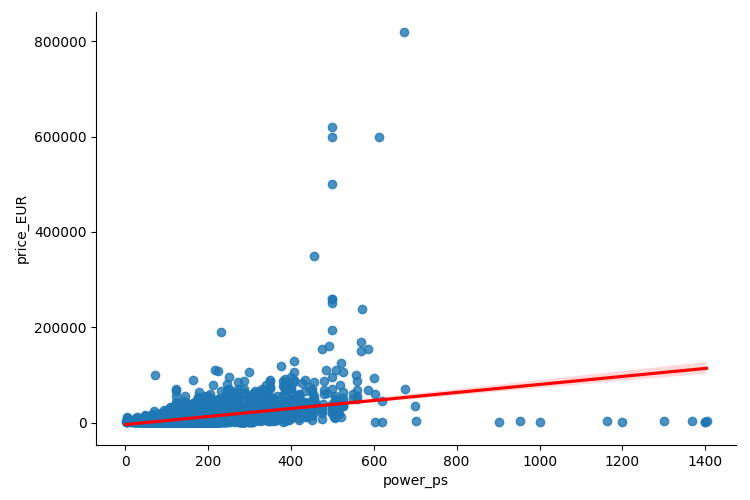
\includegraphics[scale=0.45]{Immagini/potenza}
    \caption{\textbf{Scatter Plot potenza}}
    \label{fig:power_ps}
\end{figure}
Dal grafico a dispersione soprariportato si deduce che, com'era prevedibile, il prezzo di un'auto cresce all'aumentare della sua potenza. Ciò è verificabile facilmente dall'andamento della retta di regressione.
\begin{figure}[H]
    \centering
    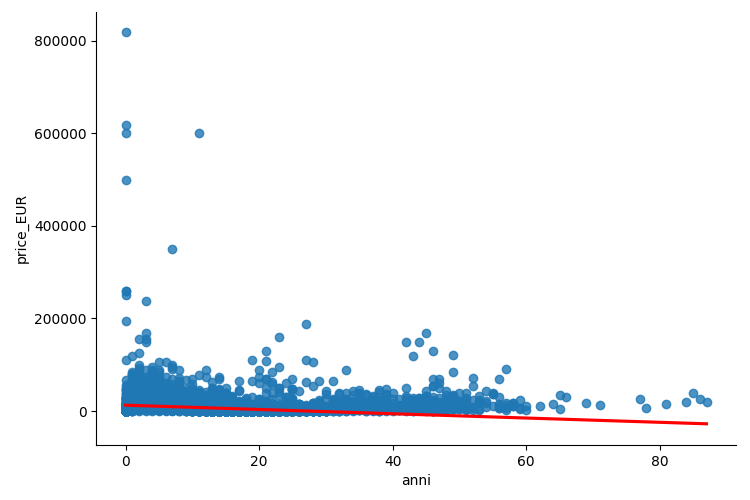
\includegraphics[scale=0.45]{Immagini/anni}
    \caption{\textbf{Scatter Plot anni}}
    \label{fig:anni}
\end{figure}
\pagebreak
Per quanto riguarda gli anni, essi sono stati ricavati dalla colonna relativa all'anno di immatricolazione del veicolo: ciò è stato fatto per rendere più chiara e naturale l'interpretazione del grafico.

Contrariamente alla potenza, il prezzo dell'auto in questo caso diminuisce all'aumentare degli anni della stessa.

\begin{figure}[H]
    \centering
    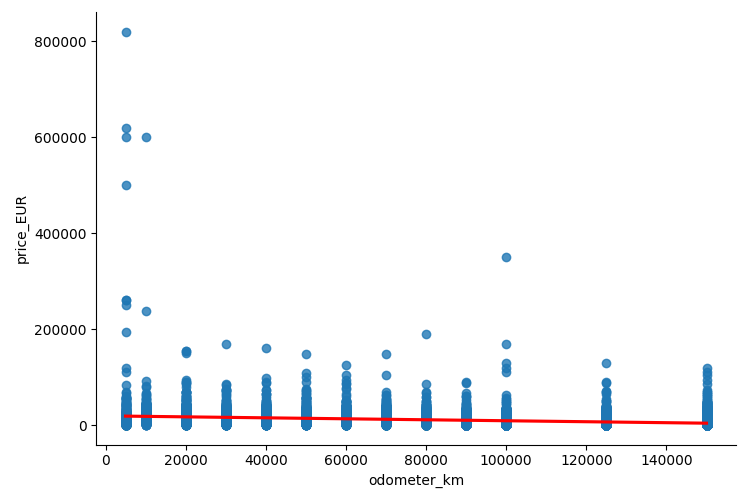
\includegraphics[scale=0.45]{Immagini/chilometraggio}
    \caption{\textbf{Scatter Plot chilometraggio}}
    \label{fig:odometer_km}
\end{figure}

Come avveniva per gli anni, ad una quantità maggiore di chilometri percorsi corrisponde un prezzo minore,
Dando un ulteriore sguardo al grafico, sembrerebbe che i valori impostati dai venditori per il chilometraggio delle proprie auto sia stato approssimato alla decina di migliaia più vicina al valore reale dei chilometri percorsi. Si potrebbe allo stesso modo approssimare il chilometraggio inserito dall'utente per effettuare la predizione.

Tra i pochi dati di tipo numerico presenti nel Dataset, questi presentavano le relazioni più interessanti. Altri (come il mese di immatricolazione) non fornivano informazioni rilevanti rispetto alla predizione del prezzo. I dati di tipo qualitativo, invece, verranno trattati diversamente nella fase di Data Preparation, dato che non è possibile visualizzarli direttamente in un grafico a dispersione.
\pagebreak

\paragraph{Possibili problemi di qualità.}
Il Dataset utilizzato non è purtroppo esente da difetti. Un esempio è il campo power\textunderscore ps (potenza): alcune istanze presentano valori superiori a 1000 CV, il che fa dedurre che probabilmente è stata inserita la cilindrata al posto della potenza. 

Un altro problema è rappresentato dal fatto che all'interno del Dataset sono presenti istanze di auto d'epoca le quali, facendo parte di un mercato completamente diverso, rischiano di influenzare negativamente la stima effettuata dal modello. 

Ciononostante non sono stati rilevati altri problemi di qualità, presumibilmente dovuto al fatto che il Dataset è stato già pulito dall'utente che l'ha caricato su Kaggle.
\medskip

\subsection{Data Preparation}

\subsection{Data Modeling}

\subsection{Evaluation}

\subsection{Deployment}